%%%%%%%%%%%%%%%%%%%%%%%%%%%%%%%%%%%%%%%%%%%%%%%%%%%
%% LaTeX book template                           %%
%% Author:  Amber Jain (http://amberj.devio.us/) %%
%% License: ISC license                          %%
%%%%%%%%%%%%%%%%%%%%%%%%%%%%%%%%%%%%%%%%%%%%%%%%%%%

\documentclass[a4paper,11pt,oneside]{book}
\usepackage[T1]{fontenc}
\usepackage[utf8]{inputenc}
\usepackage{lmodern}
\usepackage[inline,shortlabels]{enumitem}

\usepackage{hyperref}
\usepackage{graphicx}
\usepackage[english]{babel}

%%%%%%%%%%%%%%%%%%%%%%%%%%%%%%%%%%%%%%%%%%%%%%%%%%%%%%%%%%%%%%%%%%%%%%%%%%%%%%%%
% 'dedication' environment: To add a dedication paragraph at the start of book %
% Source: http://www.tug.org/pipermail/texhax/2010-June/015184.html            %
%%%%%%%%%%%%%%%%%%%%%%%%%%%%%%%%%%%%%%%%%%%%%%%%%%%%%%%%%%%%%%%%%%%%%%%%%%%%%%%%
\newenvironment{dedication}
{
   \cleardoublepage
   \thispagestyle{empty}
   \vspace*{\stretch{1}}
   \hfill\begin{minipage}[t]{0.66\textwidth}
   \raggedright
}
{
   \end{minipage}
   \vspace*{\stretch{3}}
   \clearpage
}

%%%%%%%%%%%%%%%%%%%%%%%%%%%%%%%%%%%%%%%%%%%%%%%%
% Chapter quote at the start of chapter        %
% Source: http://tex.stackexchange.com/a/53380 %
%%%%%%%%%%%%%%%%%%%%%%%%%%%%%%%%%%%%%%%%%%%%%%%%
\makeatletter
\renewcommand{\@chapapp}{}% Not necessary...
\newenvironment{chapquote}[2][2em]
  {\setlength{\@tempdima}{#1}%
   \def\chapquote@author{#2}%
   \parshape 1 \@tempdima \dimexpr\textwidth-2\@tempdima\relax%
   \itshape}
  {\par\normalfont\hfill--\ \chapquote@author\hspace*{\@tempdima}\par\bigskip}
\makeatother

%%%%%%%%%%%%%%%%%%%%%%%%%%%%%%%%%%%%%%%%%%%%%%%%%%%
% First page of book which contains 'stuff' like: %
%  - Book title, subtitle                         %
%  - Book author name                             %
%%%%%%%%%%%%%%%%%%%%%%%%%%%%%%%%%%%%%%%%%%%%%%%%%%%

% Book's title and subtitle
\title{\Huge \textbf{Artificial Intelligence}  \\ \Huge Pada Pengenalan Wajah}
\author{
  \textsc{Classroom Dev Team}
}
\begin{document}

\frontmatter
\maketitle

%%%%%%%%%%%%%%%%%%%%%%%%%%%%%%%%%%%%%%%%%%%%%%%%%%%%%%%%%%%%%%%
% Add a dedication paragraph to dedicate your book to someone %
%%%%%%%%%%%%%%%%%%%%%%%%%%%%%%%%%%%%%%%%%%%%%%%%%%%%%%%%%%%%%%%

%%%%%%%%%%%%%%%%%%%%%%%%%%%%%%%%%%%%%%%%%%%%%%%%%%%%%%%%%%%%%%%%%%%%%%%%
% Auto-generated table of contents, list of figures and list of tables %
%%%%%%%%%%%%%%%%%%%%%%%%%%%%%%%%%%%%%%%%%%%%%%%%%%%%%%%%%%%%%%%%%%%%%%%%
\tableofcontents
\listoffigures

\mainmatter

%%%%%%%%%%%%%%%%
% NEW CHAPTER! %
%%%%%%%%%%%%%%%%
\chapter{Pengantar}

\section{Artificial Intelligence Pada Pengenalan Wajah}
 Dilansir dari Stanford Computer science, Artificial Intelligence(AI) atau kecerdasan buatan adalah ilmu dan rekayasa pembuatan mesin cerdas, melibatkan mekanisme untuk menjalankan suatu tugas menggunakan komputer.  Sehingga artificial intelligence merupakan sebuah teknologi yang memungkinkan sistem komputer, perangkat lunak, program dan robot untuk “berpikir” secara cerdas layaknya manusia. Kecerdasan buatan suatu mesin dibuat oleh manusia melalui algoritma pemrograman yang kompleks.\footnote{Mustofa, Zaenal. \emph{Artificial Intelligence (AI): Pengertian, Perkembangan, Cara Kerja, Dan Dampaknya}.Universitas STEKOM} \\
\\Secara garis besar, AI dapat melakukan salah satu dari keempat faktor berikut:
\begin{enumerate}[a.]
    \item \emph{Acting Humanly} , sistem bertindak layaknya manusia.
    \item \emph{Thinking Humanly} , sistem dapat berpikir seperti manusia.
    \item \emph{Think Rationally} , sistem dapat berpikir secara rasional.
    \item \emph{Act Rationally} , sistem mampu bertindak secara rasional.
\end{enumerate}

Pengenalan dan identifikasi wajah merupakan contoh sistem penerapan konsep Artificial Intelligence menggunakan biometrik wajah yang terus berkembang pada bidang \emph{computer vision}. Kecerdasan buatan ini digunakan secara \emph{real-time} untuk menangkap dan mengenali wajah seseorang pada kamera.

Computer Vision adalah bagaimana komputer/mesin dapat melihat, teknik computer vision mampu memvisualisasikan data menganalisaberupa gambar image atau dalam bentuk vidio. Tujuan utama dari Computer Vision adalah agar komputer atau mesin dapat meniru kemampuan perseptual mata manusia dan otak, atau bahkan dapat mengunggulinya untuk tujuan tertentu.
\footnote{Wibowo, Ari.\emph{Implementasi Teknik Computer Vision}.Universitas Widyatama}

\section{Face Detection}
\emph{Face Detection} atau pengenalan wajah merupakan sebuah teknologi untuk menangkap wajah seseorang pada kamera yang menjadi tahap awal dalam sistem pengenalan wajah (\emph{Face Recognition})  yang digunakan dalam identifikasi biometrik. Deteksi wajah juga dapat digunakan untuk pencarian atau pengindeksan data wajah dari citra atau video yang berisi wajah dengan berbagai ukuran, posisi, dan latar belakang.\footnote{NUGROHO, Setyo, Drs. Agus Hardjoko, MSc.,PhD. \emph{Sistem pendeteksi wajah manusia pada citra digital}, Universitas Gajah mada, diakses dari http://etd.repository.ugm.ac.id/penelitian/detail/23416}\\

Pembuatan pendeteksi wajah ini dapat dibuat menggunakan openCV yang  merupakan aplikasi perangkat lunak untuk pengolahan citra dinamis secara \emph{real-time}, selain itu openCV juga banyak mendukung bahasa pemrograman diantaranya C++, C, python, dan java. Pada pembahasan kali ini, penjelasan mengenai proses pembuatan deteksi wajah akan menggunakan openCV dengan bahasa pemrograman python. Proses deteksi objek maupun wajah dapat menggunakan metode algoritma Haar Cascade Classifier.\\

Algoritma Haar Cascade Classifier merupakan salah satu algoritma yang digunakan untuk mendeteksi sebuah wajah dengan cepat dan \emph{real-time} sebuah benda termasuk wajah manusia. Metode ini menggunakan haar-like features dimana perlu dilakukan training terlebih dahulu untuk mendapatkan suatu pohon keputusan dengan nama cascade claasifier sebagai penentu apakah ada obyek atau tidak dalam frame yang diproses, dengan mengelompokka fitur-fitur pada gambaran wajah berdasarkan sisi yang terang dan sisi yang gelap. Adanya fitur Haar
ditentukan dengan cara mengurangi rata-rata piksel pada daerah gelap dari rata-rata piksel pada daerah terang\footnote{Suhepy Abidin.\emph{Deteksi Wajah Menggunakan Metode Haar Cascade Classifier Berbasis Webcam Pada Matlab}.Jurusan Teknik Elektro, Politeknik Negeri Ujung Pandang}


\section{Face Recognition}
Face recognition adalah sebuah teknologi yang mampu untuk mengindentifikasi dan mengkonfirmasi identitas seseorang menggunakan wajah mereka. 
Face recognition menjadi salah satu sistem identifikasi biometrik yang paling baik dalam mengindentifikasi seseorang dengan fitur-fitur khusus pada tubuh maupun DNA yang menjadi pembeda antara satu orang dengan orang lainnya. 

Menurut US Government Accountability Office, ada 4 komponen yang dibutuhkan untuk melakukan face recognition, yaitu: kamera, faceprint, Database dan terakhir Algoritme untuk membandingkan faceprint dari wajah target dengan faceprint dalam database.\footnote{Putri, Monica. \emph{Cara Kerja Face Recognition}. Universitas Binus}
Setelah terpenuhinya komponen tersebut, dilakukan beberapa tahap untuk melakukan face recognition.

Menurur Haisong Gu, Qiang Ji, dan Zhiwei Zu (2002), pengenalan wajah umumnya melalui 3 tahapan untuk mendapatkan hasil.
\begin{enumerate}[1.]
    \item \emph{Face Detection}, dilakukan untuk mendeteksi adanya atau tidak pada frame yang dibaca sistem. Pada proses ini menggunakan metode \emph{Haar-cascade Classifier}
    \item \emph{Facial Expression Information Extraction}, dilakukan pada wajah yang sudah terdeteksi untuk mengekstraksi informasi penting yang akan didapatkan dari wajah untuk membedakan wajah. Fitur atau bagain wajah yang telah diekstraksi nantinya akan digunakan untuk pencocokan wajah.
    \item \emph{Expression Clssification}, merupakan proses akhir dalam pengenalan wajah, dimana sistem melakukan pencocokan dari masukan wajah dengan data yang ada pada database
  \end{enumerate}

Ada beberapa algoritma untuk melakukan pencocokan pada proses pengenalan wajah yang disediakan oleh openCV. Local Binary Pattern Histogram (LBPH) adalah salah satu dari tiga algoritma pengenalan wajah bawaan pada library OpenCV antara lain Eigenface,
Fisherfaces, dan LBPH. Dibandingkan dengan kedua algoritma tersebut, LBPH tidak hanya dapat mengenali muka depan, tetapi juga mengenali muka samping yang lebih fleksibel. Metode ini bekerja dengan membandingkan dan mencocokan histogram yang sudah diekstraksi dengan citra wajah yang sudah ada pada database/dataset.

\newpage
\chapter{Model Algoritma  Face Recognition Pada OpenCV}
Ada beberapa model algoritma yang sudah disediakan openCV untuk melakukan pengenalan wajah, diantaranya adalah
Eigenface, Fisherfaces, dan \emph{Local binary Pattern Histogram}(LBPH). Berikut penjelasan untuk perbedaan dari ketiga model algoritma yang disediakan olen openCV.
\section{Eigenface}

Eigenface adalah salah satu algoritma pengenalan wajah yang berdasarkan
pada Principle Component Analysis (PCA) yang dikembangkan di MIT.
Algoritma EigenFace secara keseluruhan cukup sederhana, Training Image
direpresentasikan dalam sebuah vektor flat (gabungan vektor) dan digabung
bersama-sama menjadi sebuah matriks tunggal. Eigen Vector kemudian
diekstraksi dan disimpan dalam file temporary atau database. Training image
kemudian diproyeksikan dalam feature space yang di namai face space yang
ditentukan oleh eigen vektor(Mukti, 2008).\footnote{Alam, R.G guntur, dkk.\emph{MPLEMENTASI ALGORITMA EIGENFACE UNTUK FACE
RECOGNITION PADA OBJECK FOTO ID CARD}.Telematik : Vol 7, No 2, April 2015.}
%http://repository.unib.ac.id/18865/1/4.%20IMPLEMENTASI%20ALGORITMA%20EIGENFACE%20UNTUK%20FACE.pdf

Principal Component Analysis (PCA) atau disebut juga transformasi KarhunenLoeve adalah tekhnik yang digunakan untuk
menyederhanakan suatu data, dengan cara mentransormasi linear sehingga terbentuk
system koordinat baru dengan variansi maksimum. PCA dapat digunakan untuk
mereduksi dimensi suatu data tanpa mengurangi karakteristik data tersebut secara signifikan (Cahyadi, 2007: 93)
\footnote{Firliana, Lina, dkk.\emph{Implementasi Principal Component Analysis (PCA) Untuk
Pengenalan Wajah Manusia}. Universitas Nusantara}\\

Berikut proses langkah-langkah pengenalan wajah menggunakan model algoritma Eigenface.
\begin{enumerate}[1. ]
    \item Penyusunan flat vektor matriks
    \item Mengambil nilai tengah dari kumpulan matriks
    \item Menghitung selisih antara nilai matriks \emph{training image} dengan nilai tengah
    \item Menghitung nilai matriks kovarian
    \item Menghitung nilai \emph{eigenvalue} dan \emph{eigenvector}
    \item Menghitung nilai \emph{eigenface}
    \item Proses indentifikasi wajah 
\end{enumerate}

\section{Fisherfaces}

\chapter{Implementasi Sistem}
\section{Proses Instalasi}
Pembuatan sistem face detection dan face recognition akan menggunakan bahasa pemrograman Python dan \emph{library} openCV. Berikut adalah cara instalasi Python serta library openCV yang akan digunakan.

\subsection{Instalasi Python}
Instalator Python dapat didownload pada website resmi python \url{https://www.python.org/downloads}
\begin{figure}[h!]
    \centering
    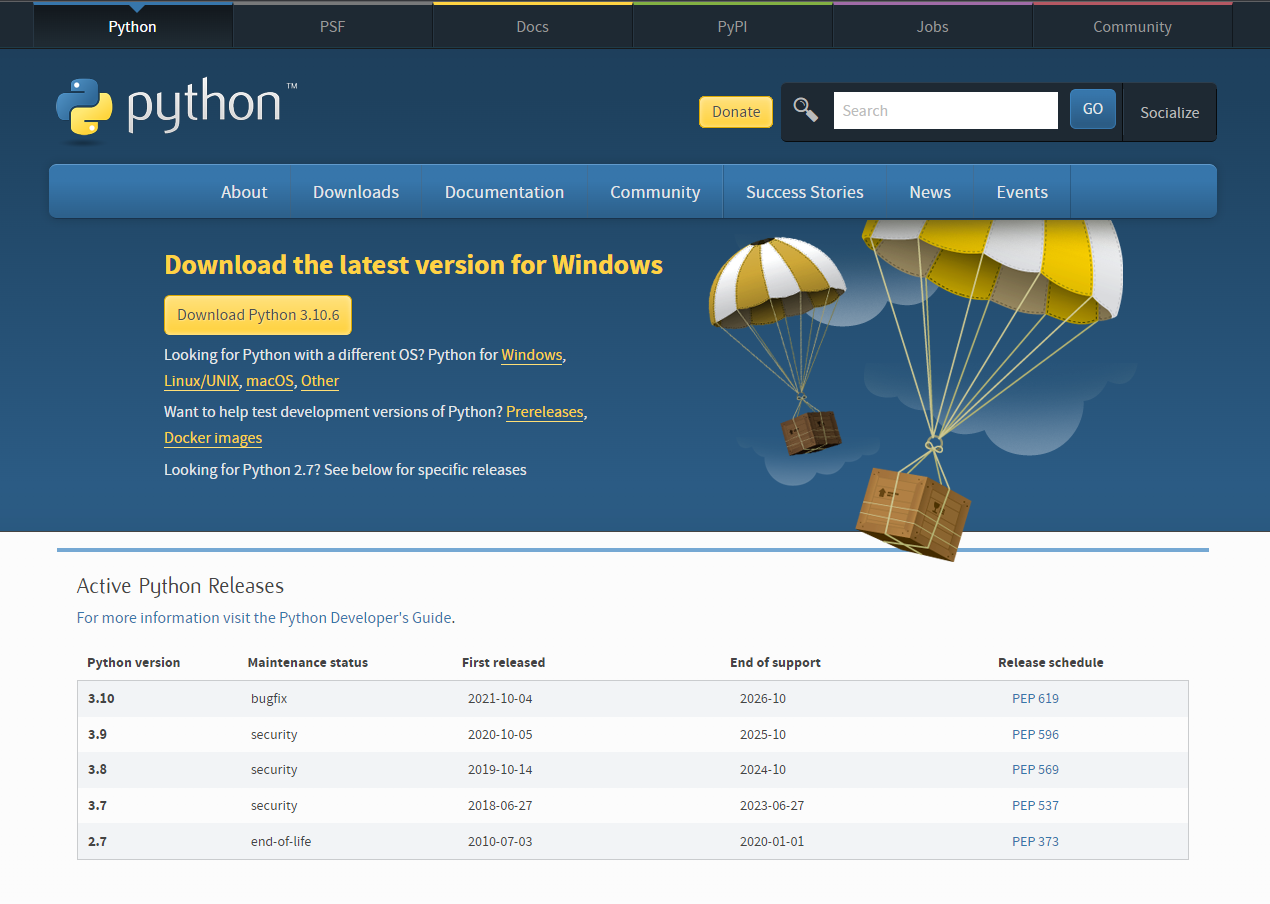
\includegraphics[width=0.9\linewidth]{images/web_py.PNG}
    \caption{Website resmi python}
\end{figure}
\\Download instalator versi terbaru dari python atau sesuaikan dengan kebutuhan penggunaan
\begin{figure}[h!]
    \centering
    
\includegraphics[width=0.9\linewidth]{images/py_ver.PNG}
    \caption{Pilihan Versi Python}
\end{figure}
\\Kemudian, buka file instalator python yang telah didownload, centang "Add Python 3.10 to PATH" dan klik \emph{Customize Installation}
\begin{figure}[h!]
    \centering
    
\includegraphics[width=0.9\linewidth]{images/py_1.PNG}
    \caption{Instalator python}
\end{figure}
\\Pilih fitur yang akan digunakan, untuk saran pilih semua fitur agar instalasi python lengkap, lalu klik 'next'
\begin{figure}[h!]
    \centering
    
\includegraphics[width=0.9\linewidth]{images/py_2.PNG}
    \caption{Pilihan fitur}
\end{figure}
\\Centang pilihan sesuai pada gambar, kemudian pilih direktori untuk lokasi penyimpanan instalasi python sesuai kebutuhan. Lalu klik "Install" dan tunggu hingga proses instalasi selesai.
\begin{figure}[h!]
    \centering
    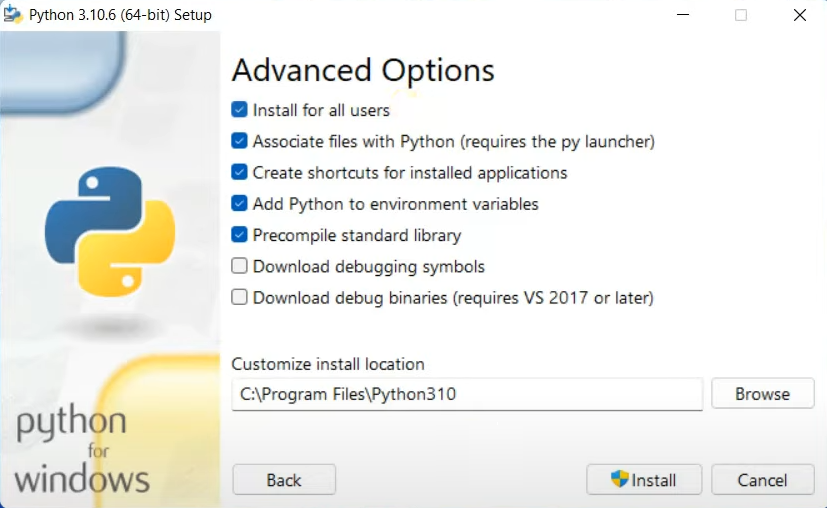
\includegraphics[width=0.9\linewidth]{images/py_3.PNG}
    \caption{Pilihan lanjutan dan penyesuaian lokasi}
\end{figure}

\subsection{Instalasi OpenCV}
Untuk Instalasi openCV dapat dilakukan melalui CMD(\emph{Command Prompt}). Buka direktori penyimpanan instalasi python, lalu menuju direktori 'Scripts' tempat pip.exe berada. Lalu tuliskan perintah \emph{pip install opencv-contrib-python} untuk memulai instalasi openCV, tunggu instalasi hingga selesai.
\begin{figure}[h!]
    \centering
    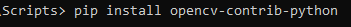
\includegraphics[width=0.7\linewidth]{images/opencv_1.PNG}
    \caption{Instalasi openCV}
\end{figure}
\\Setelah instalasi selesai, buka python IDLE atau pada CMD didalam direktori instalasi python, buka python.\\

Setelah python terbuka, ketik \textbf{import cv2} lalu enter, jika saat pengecekan openCV pada python tidak terjadi error, maka openCV berhasil di-install.
\begin{figure}[h!]
    \centering
    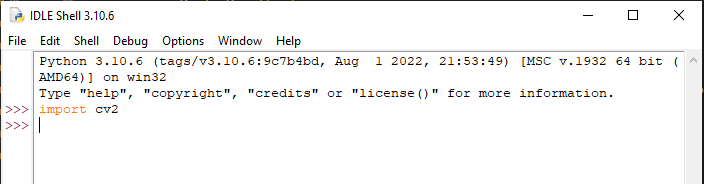
\includegraphics[width=1\linewidth]{images/opencv_2.PNG}
    \caption{Cek openCV pada python IDLE}
    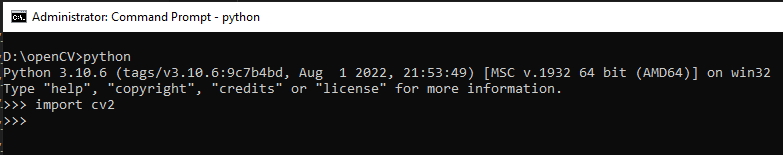
\includegraphics[width=1\linewidth]{images/opencv_3.PNG}
    \caption{Cek openCV pada CMD}
\end{figure}

\newpage
\section{Pembuatan Sistem Face Detection}
Pembuatan sistem Face Detection kali ini menggunakan algoritma Haar Cascade Classifier. Proses pertama yang dilakukan adalah dengan mengubah citra warna menjadi citra \emph{grayscale}, selanjutkan melakukan pemindaian pada citra \emph{grayscale} untuk mendapatkan nilai fitur citra dengan \emph{Haar-Like Feature} yang menyatakan objek wajah.\\

Berikut ini merupakan bagian-bagian untuk membuat sistem face detection atau pendeteksi wajah.\\
\\- Memasukan library, \textbf{cv2} = merupakan \emph{library} openCV
\begin{figure}[h!]
    \centering
    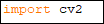
\includegraphics[width=0.3\linewidth]{images/1.PNG}
    \caption{Memasukan library openCV}
\end{figure}
\\- Proses face detection, untuk melakukan proses deteksi wajah akan menggunakan algoritma \emph{haarcascade}. Dengan fungsi \textbf{cv2.CascadeClassifier}
\begin{figure}[h!]
    \centering
    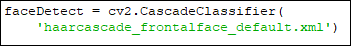
\includegraphics[width=0.7\linewidth]{images/2.PNG}
    \caption{Memasukan library openCV}
\end{figure}
\\- Memasukan video, \textbf{cv2.VideoCapture} merupakan fungsi untuk membaca video yang akan dijadikan \emph{sample} dan bisa juga untuk menampilkan frame kamera yang terkoneksi dengan komputer.
\begin{figure}[h!]
    \centering
    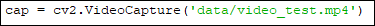
\includegraphics[width=0.7\linewidth]{images/3.PNG}
    \caption{Memasukan video}
\end{figure}
\\- Membuka video/kamera dan merubah warna. Kode pada baris pertama digunakan untuk membuka video atau kamera yang terhubung, baris kedua merupakan
kode untuk mengubah warna citra menjadi hitam putih menggunakan \textbf{cv2.cvtColor}
\begin{figure}[h!]
    \centering
    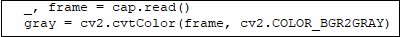
\includegraphics[width=0.7\linewidth]{images/4.PNG}
    \caption{Membuka video dan ubah warna cira}
\end{figure}
\\- Fungsi untuk mendeteksi wajah, menggunakan fungsi \textbf{detectMultiScale}
\begin{figure}[h!]
    \centering
    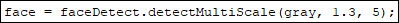
\includegraphics[width=0.7\linewidth]{images/5.PNG}
    \caption{Deteksi wajah}
\end{figure}
\\- Fungsi untuk membuat bingkai tanda jika wajah terdeteksi oleh sistem menggunakan \textbf{cv2.rectangle} jika berbentuk persegi. Dan fungsi \textbf{cv2.imshow} untuk menjalankan sistem yang telah dibuat.
\begin{figure}[h!]
    \centering
    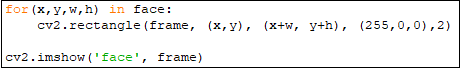
\includegraphics[width=0.75\linewidth]{images/6.PNG}
    \caption{Kode bingkai wajah}
\end{figure}
\\Berikut adalah seluruh kode dan hasil untuk sistem deteksi wajah:
\begin{figure}[h!]
    \centering
    \includegraphics[width=0.75\linewidth]{images/full.PNG}
    \caption{Kode deteksi wajah}
\end{figure}
\begin{figure}[h!]
    \centering
    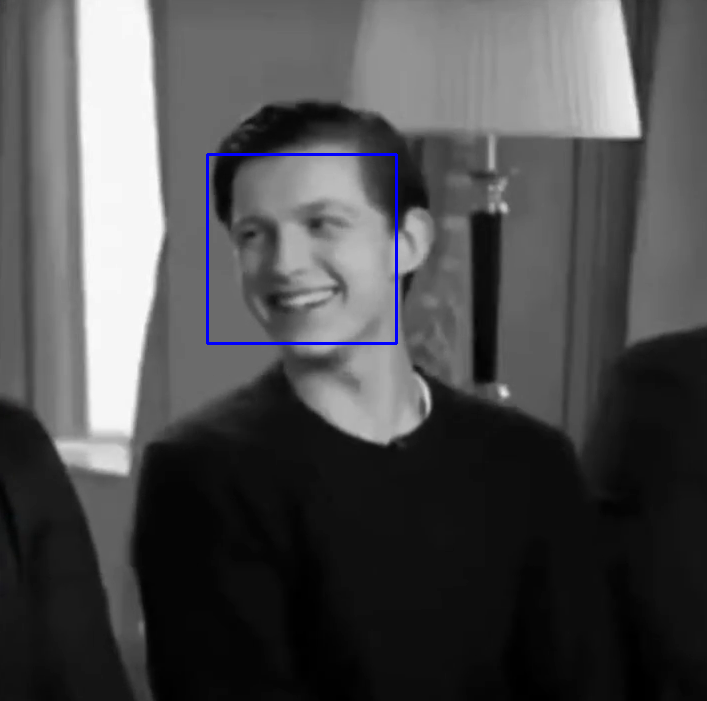
\includegraphics[width=0.33\linewidth]{images/HASIL 1.PNG}
    \includegraphics[width=0.34\linewidth]{images/HASIL 2.PNG}
    \caption{Hasil deteksi wajah}
\end{figure}

\newpage
\section{Pembuatan Sistem Face Recognition}
Prose pertama untuk melakukan pengenalan wajah yaitu dengan mengumpulkan dataset yang akan di \emph{training} dengan menangkap citra wajah pada saat awal deteksi wajah yang akan disimpan dan dikumpulkan berdasarkan id yang telah dimasukkan user. Setelah dataset terkumpul, selanjutnya
sistem akan melakukan \emph{training data} untuk mengenali wajah berdasarkan id. Kemudian proses penenalan wajah pun dilakukan dengan mendeteksi wajah mengunakan algoritma Haar-cascade classifier, lalu sistem akan melakukan pencocokan dengan menggunakan fitur LBPH untuk mencocokan wajah yang terdeteksi dengan dataset yang sudah di\emph{training} sebelumnya.
\begin{enumerate}[- ]
\item Mengumpulkan dataset dengan metode \emph{Haar-cascade classifier}
\item Proses training dataset
\item Proses pengenalan wajah dengan metode \emph{Local Binary Patter Histogram(LBPH)}
\item Testing aplikasi
\end{enumerate}


\end{document}
